%
%Latex Document made by Team HotPink for SRS,  Round 1,  Assignment 1,  COS 301 2017
%

\documentclass[11pt, a4paper]{article}
\usepackage{geometry}
 \geometry{
 a4paper, 
 total={170mm, 257mm}, 
 left=25mm, 
right=25mm, 
 top=25mm, 
 }

\title{Software Requirements Specification \\ NavUP \\ COS 301 \\ Team: Hotpink}
\date{Friday,  February 24,  2017}
\author{Gregory Austin 14039712 \\ Stephanie Groutsch 14293324 \\ Timothy Kirker 11152402 \\ Drew Langley 11039753 \\ Xoliswa Ntshingila 13410378
\\ Melvin Zitha 12138747}


\usepackage[latin1]{inputenc}
\usepackage{amsmath}
\usepackage{amsfonts}
\usepackage{amssymb}
\usepackage{graphicx}
\usepackage{float}

\DeclareGraphicsExtensions{.png}
\DeclareGraphicsExtensions{.jpg}

%\usepackage{fullpage}

\begin{document}
\maketitle
\newpage
\tableofcontents
%insert table of contents and figues etc

	%%%%%%%%%%%%%%%%%%%%%%%%%%%%%%%%%%%%%%%%%%%%%%%%%%%%%%%%%%%%%%%%%%%%%%%%%%%%%%
	%%%%%%%%%%%%%%%%%%%%%%%		INTRODUCTION	     %%%%%%%%%%%%%%%%%%%%%%%%%%%%%%%%%%%%%%%%%%
	%%%%%%%%%%%%%%%%%%%%%%%%%%%%%%%%%%%%%%%%%%%%%%%%%%%%%%%%%%%%%%%%%%%%%%%%%%%%%%
\newpage
\section{Introduction}
	\subsection{Purpose}
	The purpose of this document is to provide a detailed description of the requirements for the NavUP application,  a navigation application which is intended to assist students,  staff and the  public with navigating the University of Pretoria. Additionally it will outline and explain the complete plan for building the NavUP system.The explanations include the constraints for the system and how the system will interact with external applications. Ultimately this document is to be used for client approval such that the system may be implemented.

	\subsection{Scope}

		The NavUP mobile application makes use of the Wi-Fi on campus in order to assist the user in finding the route to their destination from their current location or from a location which is on the University of Pretoria facilities this includes but is not limited to lecture halls,  food courts,  ablution facilities or possibly even sport or faculty houses. 
		\\
		The NavUP mobile application will use the users GPS location,  on their smart devices,  in conjunction with all the Wi-Fi routers on campus in order to determine the best route from their starting location. As a result the users require Wi-Fi enabled devices and login credentials to the Universities Wi-Fi network.The system will not be able to navigate a user from a location which is 			not within the range of the campus Wi-Fi.
		\\
 		Further more the  NavUP system also includes best route capabilities,  optimal routes for users with disabilities,  status of the number of people currently on campus based on the number of devices currently connected to the Wi-Fi network, points of interest,  activities and events that are happening on campus. It will also track the activity of the user e.g. The number of steps 				taken and reward the user based on the goals  they have achieved.

	\subsection{Overview}
		These are the chapters that follow; The Overall description chapter which describes the overall system,  the modules and the interfaces that exist within the system,  the system functions,  the charecteristics of the users of the system and the system constraints. The Specific Requirements chapter is intended for developers and contains the external interface requirements,  			functional requirements,  performance capabilities of the system as well as the design constraints and quality related requirements.

	%%%%%%%%%%%%%%%%%%%%%%%%%%%%%%%%%%%%%%%%%%%%%%%%%%%%%%%%%%%%%%%%%%%%%%%%%%%%%%
	%%%%%%%%%%%%%%%%%%%%%%%		OVERALL DESCRIPTION	     %%%%%%%%%%%%%%%%%%%%%%%%%%%%%%%%%%%%%%%
	%%%%%%%%%%%%%%%%%%%%%%%%%%%%%%%%%%%%%%%%%%%%%%%%%%%%%%%%%%%%%%%%%%%%%%%%%%%%%%
\newpage
\section{Overall Description}
	\subsection{Product Perspective}
	Similar to existing navigation applications such as: Google Maps,  Apple Maps and Waze,  NavUP is a standalone mobile application that acts as a campus navigation system which will be open for all UP students,  staff and guests to use. It encompasses all technologies,  which will be required for the necessary functionality as described in the product functions section. 
	\\
	\par
The application will be implented using the relevant,   already existing hardware,   software interfaces,  OS interfaces and technologies such as,  Wi-Fi,  Cellular Data and GPS. Implementation of the hardware interfaces will require the  existing software interfaces/OS interfaces to access data from the hardware interfaces relating to the main functionality of the NavUP application. 
	\\
	\par
The application will use communication interfaces to determine traffic and the best routes to follow,  these communication interfaces will work through the required hardware interfaces. The main operations of the application will be accessed through the user interface,  which will utilize underlying  technologies. These operations include: navigating to a class,   providing direction (showing where to go), displaying destination information( describing where and what it is you're going to). The DBMS will have to be manually maintained with location and event data or interfaced with an existing DBMS / DSS that the university already has. 

	\subsection{Product Functions}
	The NavUP mobile application will support a variety of functions namely; navigation,  providing information,  allowing for users to decide on different routes,  achieving goals and personalisation capabilities.
	\\

	The navigation functionality will consist of locating the user and then navigating them to their required location. They will be provided with searching capabilities in order to obtain their required location. Users will then be able to save their destination for future use.
	\\

	Information will be provided to users when they are near points of interest. This information will consist of historical and general information regarding venues and/or landmarks. Information regarding cultural and sporting events that relate to the user will also be shown when appropriate.
	\\

	Different routes will be provided based on the users needs. Such routes will include the fastest path from one location to the next. This path will be determined based on the amount of pedestrian traffic. Another route will be provided for users with special needs in order to allow them to reach their destination using the most user friendly path for their disability.
	\\

	Weekly goals will be provided to motivate users to attend all their lectures during the week,  explore the campus and be more informed about it as well as to increase the amount of steps they take this being beneficial to their overall wellbeing.

	\subsection{User Characteristics}
	There are three main categories of individuals that will make use of the application namely administrators,  general users and third party rewards managers.
	\\


	The administrators will ensure that the software works as intended and will be in charge of maintaining and upgrading the application. These users will need to understand how the system works as well as have programming knowledge in order to work on the software.
	\\

	The general users of the system will consist of students,  lecturers,  guests and university employees. They will only make use of the mobile application. This means that they will not require any knowledge of how the software is implemented however,  they will need to have knowledge regarding how to use a smart device. These users will mainly use the application for navigational purposes.
	\\

	Third party rewards managers will consist of business parties who will provide rewards to individuals who have obtained their weekly goal. Since they will only make use of the client side of the mobile application, they will not require any knowledge of how the system is implemented. They will however, require knowledge regarding whether the user has reached their goal or not.

	\subsection{Constraints}
	The following are restrictions related to the application:
		\begin{enumerate}
				\renewcommand{\labelenumi}{{\textbf{\arabic{enumi}.}}}
				\item Security  - The users personal information and current location should not be accessible to the public.
				\item Accuracy - The users location should be found whether the user is indoors or not. The location of the user should also be found in terms of which floor they are on in the building.
				\item Performance - The system should be able to handle a large amount of users making use of the software at the same time.
				\item Reliability - The application should still operate when one or more data access points are no longer available.
				\item Accessibility - The application should be easily accessible to everyone that requires it.
				\item Usability - The applications interface should be easy to use and understand.
				\item Size - The application should not require too much memory in order to operate.
				\end{enumerate}
	\newpage
	\subsection{Assumptions and Dependencies}
	Since the NavUP system is being created for mobile devices,  it is assumed that all those who require the application,  will have access to a mobile device. It is then assumed that these devices will have the required capabilities necessary to run the application. Such dependencies include built in WiFi,  GPS and cellular connectivity as well as the required data/airtime(in the event that they are not connected to the University's Wi-Fi).
\\
\par
Assumed users will be registered students of the University of Pretoria thereby having access to their modules and class data for navigating when required with minimal input from the user, this depends on access to students data for the DBMS, staff navigating to their work stations , guests wanting to navigate to a location which they only know by name.
\\
\par
In terms of the usability of the application,  it is assumed that users will have knowledge regarding how to use mobile devices and applications on such devices such as the downloading and installation of applications to a smart device.
\\
\par
The assumption relating to accuracy includes the belief that the application will be up to date with the latest information in terms of venues,  landmarks and events. This assumes that there will always be someone maintaining and updating the applications data,  or a DBMS that is interfaced with the university DBMS.  
\\
\par
An assumption in terms of the systems performance includes the idea that it will still be able to function when a large amount of users are making use of the application at the same time. This depends on server capacity as well as solid code structures that are efficient as well as secure.

	
	%%%%%%%%%%%%%%%%%%%%%%%%%%%%%%%%%%%%%%%%%%%%%%%%%%%%%%%%%%%%%%%%%%%%%%%%%%%%%%
	%%%%%%%%%%%%%%%%%%%%%%%		REQUIREMENTS SPECIFICATION	     %%%%%%%%%%%%%%%%%%%%%%%%%%%%%%%%%%%%
	%%%%%%%%%%%%%%%%%%%%%%%%%%%%%%%%%%%%%%%%%%%%%%%%%%%%%%%%%%%%%%%%%%%%%%%%%%%%%%
\newpage
\section{Requirements Specification}		
		
		The NavUP system will be available for use on many platforms and make use of multiple means of newtork links and other extenal interfaces such as GPS and GIS services.
		Other requirements such as quality,  integration and architectural constraints will also be covered in this section.
		
	\subsection{Functional Requirements Specification}
	%%%%%%%%%%%%%%%%%%%%%%======================   REQUIREMENTS    ================%%%%%%%%%%%%%%%%
	\subsubsection{Requirements}
		
		\subsubsection {REQ1: Navigation}
			Provide navigation functionality.
			
		\subsubsection {REQ2: Provide Information}
			Provide information regarding points of interest and sporting and cultural activities.
			
		\subsubsection{REQ3: Provide Different Routes}
			Provide different routes based on the user's needs and preferences.
		
		\subsubsection{REQ4: User Profiles}
			The system should allow users and administrators login capability.
			
		\subsubsection{REQ5: Weekly goals}
			Provide weekly goals based on the number of steps or distance travelled by the user.
			
		\subsubsection{REQ6: Personalization}
			Users should be allowed to save personalized information as well as retrieve it.
			
		\subsubsection{REQ7: Maintenance}
			The system should allow administrators the ability to C.R.U.D it.
			
%%%%%%%%%%%%%%%%%%%%%%======================   USE CASES   ================%%%%%%%%%%%%%%%%
	\newpage
	\subsection{Use Cases}
	%%%%%%%%%%%%%%%%%%%%%%======================   UC1    ================%%%%%%%%%%%%%%%%
		\subsubsection{Use Case for REQ1: Navigate user to their desired location}
			\begin{enumerate}
			\renewcommand{\labelenumi}{{\textbf{\arabic{enumi}.}}}
			\item Use Case ID: UC1
			\item Precondition: User is running the NavUP application and enters the navigation module
			\item Postcondition: Client device recieves and displays navigational information to destination.
			\item Actor-System interaction model:
				\graphicspath{ {./Images/User/} }
				\begin{figure}[h]
				\caption{Use Case Diagram -  UC1 Navigate user to their desired location}
				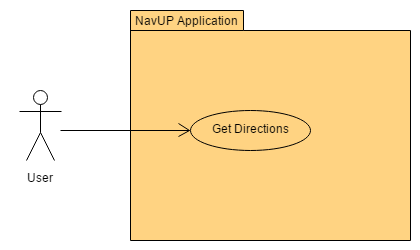
\includegraphics[height = 200px]{GetDesiredLocation.png}
				\end{figure}
			\end{enumerate}

		\begin{table}[htb]
			\centering
			\caption{UC1 -  Navigate user to their desired location}
			\label{my-label}
			\begin{tabular}{|l|l|}
				\hline
				\textbf{Actor: User} &
				\textbf{System: NavUP}
				 \\ \hline  & 0. The NavUP system displays the main window
				\\ \hline
				\begin{tabular}[c]{@{}l@{}}1. The user clicks on the navigation \\ button in the main menu\end{tabular}       &
				\begin{tabular}[c]{@{}l@{}}2. The system displays the navigation page to \\ the user\end{tabular}
				 \\ \hline
				\begin{tabular}[c]{@{}l@{}}3. The user clicks on the Get Directions button\\ on the Navigation page\end{tabular} & 
				\begin{tabular}[c]{@{}l@{}}4. The system prompts the user for their \\ required destination\end{tabular}
				\\ \hline
				5. User enters desired destination & 
				\begin{tabular}[c]{@{}l@{}}6. The system calculates and displays the route\\ and directions to the destination\end{tabular}
				\\ \hline
			\end{tabular}
		\end{table}

		
		
		%%%%%%%%%%%%%%%%%%%%%%======================   UC2    ================%%%%%%%%%%%%%%%%
		\newpage
		\subsubsection{Use Case for REQ1: Obtain Current Location}
			\begin{enumerate}
			\renewcommand{\labelenumi}{{\textbf{\arabic{enumi}.}}}
			\item Use Case ID: UC2
			\item Precondition: User is running the NavUP application and requires their location
			\item Postcondition: Client device recieves and displays the user's current location data.
			\item Actor-System interaction model:
				\graphicspath{ {./Images/User/} }
				\begin{figure}[h]
				\caption{Use Case Diagram -  UC2  Obtain Current Location}
				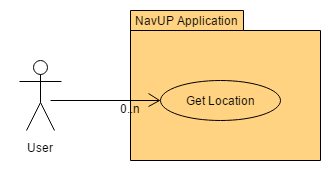
\includegraphics[height = 200px]{ObtainCurrentLocation.png}
				\end{figure}
			\end{enumerate}

		\begin{table}[htb]
			\centering
			\caption{UC2 -  Obtain Current Location}
			\label{my-label}
			\begin{tabular}{|l|l|}
				\hline
				\textbf{Actor: User} &
				\textbf{System: NavUP}
				 \\ \hline  & 0. The NavUP system displays the main window
				\\ \hline
				\begin{tabular}[c]{@{}l@{}}1. The user clicks on the navigation \\ button in the main menu\end{tabular}       &
				\begin{tabular}[c]{@{}l@{}}2. The system displays the navigation page to \\ the user\end{tabular}
				 \\ \hline
				\begin{tabular}[c]{@{}l@{}}3. The user clicks on the Get Location button\\ on the Navigation page\end{tabular} & 
				\begin{tabular}[c]{@{}l@{}}4. The system displays the user's location
				\end{tabular}
				\\ \hline
			\end{tabular}
		\end{table}
		
		
		%%%%%%%%%%%%%%%%%%%%%%======================   UC3    ================%%%%%%%%%%%%%%%%
		\newpage
		\subsubsection{Use Case for REQ1: Search for Location}
			\begin{enumerate}
			\renewcommand{\labelenumi}{{\textbf{\arabic{enumi}.}}}
			\item Use Case ID: UC3
			\item Precondition: User is running the NavUP application and searches for a given location.
			\item Postcondition: Information regarding  the searched location os provided.
			\item Actor-System interaction model:
				\graphicspath{ {./Images/User/} }
				\begin{figure}[h]
				\caption{Use Case Diagram -  UC3  Search for location}
				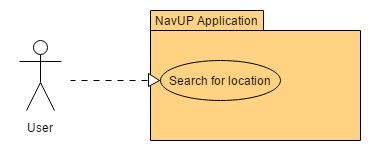
\includegraphics[height = 200px]{SearchForLocation.png}
				\end{figure}
			\end{enumerate}

		\begin{table}[htb]
			\centering
			\caption{UC3 -  Search for location}
			\label{my-label}
			\begin{tabular}{|l|l|}
				\hline
				\textbf{Actor: User} &
				\textbf{System: NavUP}
				 \\ \hline  & 0. The NavUP system displays the main window
				\\ \hline
				\begin{tabular}[c]{@{}l@{}}1. The user clicks on the navigation \\ button in the main menu\end{tabular}       &
				\begin{tabular}[c]{@{}l@{}}2. The system displays the navigation page to \\ the user\end{tabular}
				 \\ \hline
				\begin{tabular}[c]{@{}l@{}}3.  The user clicks on the Search for Location\\ button on the Navigation page\end{tabular} & 
				\begin{tabular}[c]{@{}l@{}}4. The system prompts the user for the \\ location they wish to search\end{tabular}
				\\ \hline
				5. User enters desired location & 
				\begin{tabular}[c]{@{}l@{}}6. The system provides information regarding \\ the searched location\end{tabular}
				\\ \hline
			\end{tabular}
		\end{table}

		
		%%%%%%%%%%%%%%%%%%%%%%======================   UC4    ================%%%%%%%%%%%%%%%%
		\newpage
		\subsubsection{Use Case for REQ1: Calculate the estimated time of arrival}
			\begin{enumerate}
			\renewcommand{\labelenumi}{{\textbf{\arabic{enumi}.}}}
			\item Use Case ID: UC4
			\item Precondition: User is running the NavUP application and currently travelling to a destination.
			\item Postcondition: Client device recieves and displays the estimated time of arrival.
			\item Actor-System interaction model:
				\graphicspath{ {./Images/User/} }
				\begin{figure}[h]
				\caption{Use Case Diagram - UC4  Calculate the estimated time of arrival}
				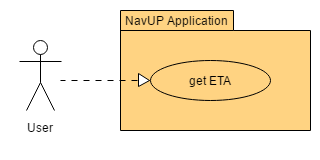
\includegraphics[height = 200px]{CalculateETA.png}
				\end{figure}
			\end{enumerate}

		\begin{table}[htb]
			\centering
			\caption{UC4 - Calculate the estimated time of arrival}
			\label{my-label}
			\begin{tabular}{|l|l|}
				\hline
				\textbf{Actor: User} &
				\textbf{System: NavUP}
				 \\ \hline  & 0. The NavUP system displays the main window
				\\ \hline
				\begin{tabular}[c]{@{}l@{}}1. The user clicks on the navigation \\ button in the main menu\end{tabular}       &
				\begin{tabular}[c]{@{}l@{}}2. The system displays the navigation page to \\ the user\end{tabular}
				 \\ \hline
				\begin{tabular}[c]{@{}l@{}}3. The user clicks on the Estimated Time of \\Arrival button on the Navigation page\end{tabular} & 
				\begin{tabular}[c]{@{}l@{}}4. The system displays the estimated time \\of arrival to the user\end{tabular}
				\\ \hline
			\end{tabular}
		\end{table}

		%%%%%%%%%%%%%%%%%%%%%%======================   UC5    ================%%%%%%%%%%%%%%%%
		\newpage
		\subsubsection{Use Case for REQ2: Display metadata with information regarding venues and points of interest}
			\begin{enumerate}
			\renewcommand{\labelenumi}{{\textbf{\arabic{enumi}.}}}
			\item Use Case ID: UC5
			\item Precondition: User is running the NavUP application and is currently travelling to a destination.
			\item Postcondition: Client device displays a popup of information a point(s)of interest.
			\end{enumerate} 

		\begin{table}[htb]
			\centering
			\caption{UC5 - Display metadata with information regarding venues and points of interest}
			\label{my-label}
			\begin{tabular}{|l|l|}
				\hline
				\textbf{Actor: User} &
				\textbf{System: NavUP}
				 \\ \hline  & 0. The NavUP system displays the main window
				\\ \hline
				\begin{tabular}[c]{@{}l@{}}1. The user travels past a point of interest\\ or venue\end{tabular}       &
				\begin{tabular}[c]{@{}l@{}}2. The system displays information related to the\\point of interest or venue to the user\end{tabular}
				\\ \hline
			\end{tabular}
		\end{table}
		
		%%%%%%%%%%%%%%%%%%%%%%======================   UC6    ================%%%%%%%%%%%%%%%%
		\subsubsection{Use Case for REQ2: Provide information regarding sports and cultural activities}
			\begin{enumerate}
			\renewcommand{\labelenumi}{{\textbf{\arabic{enumi}.}}}
			\item Use Case ID: UC6
			\item Precondition: The user is running the application and requests to view activities.
			\item Postcondition: Client device recieves and displays information regarding the requested activities.
			\item Actor-System interaction model:
				
			\end{enumerate}

		\begin{table}[htb]
			\centering
			\caption{UC6 -  Provide information regarding sports and cultural activities}
			\label{my-label}
			\begin{tabular}{|l|l|}
				\hline
				\textbf{Actor: User} &
				\textbf{System: NavUP}
			 \\ \hline  & 0. The NavUP system displays the main window
				\\ \hline
				\begin{tabular}[c]{@{}l@{}}1. The user clicks the Activities button on \\the main menu\end{tabular}       &
				\begin{tabular}[c]{@{}l@{}}2. The system displays information regarding\\ sporting and cultural activities that relate to \\the user\end{tabular}
				\\ \hline
			\end{tabular}
		\end{table}
	
		%%%%%%%%%%%%%%%%%%%%%%======================   UC7    ================%%%%%%%%%%%%%%%%
		\subsubsection{Use Case for REQ3: Provide special routes for users with disabilities}
			\begin{enumerate}
			\renewcommand{\labelenumi}{{\textbf{\arabic{enumi}.}}}
			\item Use Case ID: UC7
			\item Precondition: The user is running the application and requires a special route as they have a disability.
			\item Postcondition: Client device recieves and displays information regarding the optimal navigational route for the special needs user.
			\item Actor-System interaction model:
				\graphicspath{ {./Images/User/} }
				\begin{figure}[h]
				\caption{Use Case Diagram - UC7  Provide special routes for users with disabilities}
				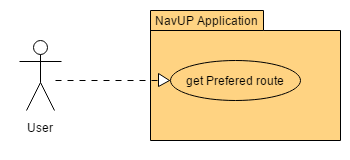
\includegraphics[height = 200px]{getPreferedRoute.png}
				\end{figure}
			\end{enumerate}

		\begin{table}[htb]
			\centering
			\caption{UC7 -  Provide special routes for users with disabilities}
			\label{my-label}
			\begin{tabular}{|l|l|}
				\hline
				\textbf{Actor: User} &
				\textbf{System: NavUP}
				 \\ \hline  & 0. The NavUP system displays the main window
				\\ \hline
				\begin{tabular}[c]{@{}l@{}}1. The user clicks the Routes button on \\the main menu\end{tabular}       &
				\begin{tabular}[c]{@{}l@{}}2. The system prompts the user for \\ a destination\end{tabular}
				\\ \hline
				\begin{tabular}[c]{@{}l@{}}3. The user enters a destination\end{tabular}       &
				\begin{tabular}[c]{@{}l@{}}4. The system prompts the user for \\ the type of route they require\end{tabular}
				\\ \hline
				\begin{tabular}[c]{@{}l@{}}5. The user selects the ''special needs'' option\end{tabular}       &
				\begin{tabular}[c]{@{}l@{}}6. The system displays the route and directions\\ to the destination.\end{tabular}
				\\ \hline
			\end{tabular}
		\end{table}

		%%%%%%%%%%%%%%%%%%%%%%======================   UC8    ================%%%%%%%%%%%%%%%%
		\newpage
		\subsubsection{Use Case for REQ3: Provide the fastest route to a destination}
			\begin{enumerate}
			\renewcommand{\labelenumi}{{\textbf{\arabic{enumi}.}}}
			\item Use Case ID: UC8
			\item Precondition: The user running the application and requires the fastest route from one location to the next.
			\item Postcondition: Client device recieves and displays information regarding the optimal navigational route.
			\item Actor-System interaction model:
				\graphicspath{ {./Images/User/} }
				\begin{figure}[h]
				\caption{Use Case Diagram - UC8  Providethe fastest route to a destination}
				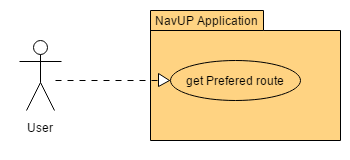
\includegraphics[width = 300px]{getPreferedRoute.png}
		\end{figure}
			\end{enumerate}

		\begin{table}[htb]
			\centering
			\caption{UC8 -  Provide the fastest route to a destination}
			\label{my-label}
			\begin{tabular}{|l|l|}
				\hline
				\textbf{Actor: User} &
				\textbf{System: NavUP}
			 \\ \hline  & 0. The NavUP system displays the main window
				\\ \hline
				\begin{tabular}[c]{@{}l@{}}1. The user clicks the Routes button on \\the main menu\end{tabular}       &
				\begin{tabular}[c]{@{}l@{}}2. The system prompts the user for \\ a destination\end{tabular}
				\\ \hline
				\begin{tabular}[c]{@{}l@{}}3. The user enters a destination\end{tabular}       &
				\begin{tabular}[c]{@{}l@{}}4. The system prompts the user for \\ the type of route they require\end{tabular}
				\\ \hline
				\begin{tabular}[c]{@{}l@{}}5. The user selects the ''fastest path'' option\end{tabular}       &
				\begin{tabular}[c]{@{}l@{}}6. The system displays the route and\\directions to the destination.\end{tabular}
				\\ \hline
			\end{tabular}
		\end{table}
		
		%%%%%%%%%%%%%%%%%%%%%%======================   UC9    ================%%%%%%%%%%%%%%%%
		\newpage
		\subsubsection{Use Case for REQ4: The user logs into the application}
			\begin{enumerate}
			\renewcommand{\labelenumi}{{\textbf{\arabic{enumi}.}}}
			\item Use Case ID: UC9
			\item Precondition: The user wishes to log into the application.
			\item Postcondition: Client device logs the user into the system and displays the user's login page.
			\item Actor-System interaction model:
				\graphicspath{ {./Images/User/} }
				\begin{figure}[h]
				\caption{Use Case Diagram -  UC9 The user logs into the application}
				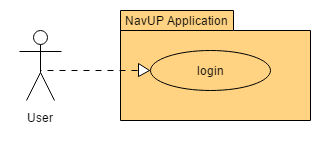
\includegraphics[height = 200px]{Login.png}
				\end{figure}
			\end{enumerate}

		\begin{table}[htb]
			\centering
			\caption{UC9 - The user logs into the application}
			\label{my-label}
			\begin{tabular}{|l|l|}
				\hline
				\textbf{Actor: User} &
				\textbf{System: NavUP}
				 \\ \hline  & 0. The NavUP system displays the main window
				\\ \hline
				\begin{tabular}[c]{@{}l@{}}1. The user clicks the Login button on \\the main menu\end{tabular}       &
				\begin{tabular}[c]{@{}l@{}}2. The system prompts the user to\\ enter the required login details\end{tabular}
				\\ \hline
				\begin{tabular}[c]{@{}l@{}}3. The user enters their login information\end{tabular}       &
				\begin{tabular}[c]{@{}l@{}}4. The system logs the user into the\\ application and displays the user's user page\end{tabular}
				\\ \hline
			\end{tabular}
		\end{table}

		%%%%%%%%%%%%%%%%%%%%%%======================   UC10    ================%%%%%%%%%%%%%%%%
		\newpage
		\subsubsection{Use Case for REQ5: Collecting and viewing rewards}
			\begin{enumerate}
			\renewcommand{\labelenumi}{{\textbf{\arabic{enumi}.}}}
			\item Use Case ID: UC10
			\item Precondition: The user is logged in and completes an activity.
			\item Postcondition: Client device recieves a notification concerning the completion of and activity and is directed to the third party rewards system.
			\item Actor-System interaction model:
				\graphicspath{ {./Images/User/} }
				\begin{figure}[h]
				\caption{Use Case Diagram - UC10 Collecting and viewing rewards}
				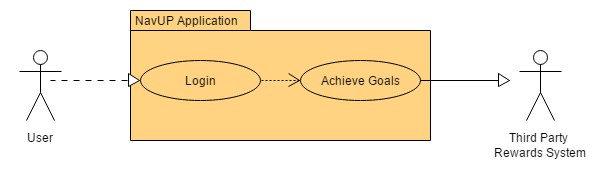
\includegraphics[width = 500px]{GetRewards.png}
				\end{figure}
			\end{enumerate}

		\begin{table}[htb]
			\centering
			\caption{UC10 - Collecting and viewing rewards}
			\label{my-label}
			\begin{tabular}{|l|l|}
				\hline
				\textbf{Actor: User} &
				\textbf{System: NavUP}
				 \\ \hline  & 0. The NavUP system displays the user's page
				\\ \hline
				\begin{tabular}[c]{@{}l@{}}1. The user completes an activity\end{tabular}       &
				\begin{tabular}[c]{@{}l@{}}2. The system notifies the user concerning\\ the completion of an activity and directs\\ the user to the third party rewards \\system \end{tabular}
				\\ \hline
			\end{tabular}
		\end{table}

		
		%%%%%%%%%%%%%%%%%%%%%%======================   UC11    ================%%%%%%%%%%%%%%%%
		\newpage
		\subsubsection{Use Case for REQ6: Allow users the ability to save a location(drop a pin)}
			\begin{enumerate}
			\renewcommand{\labelenumi}{{\textbf{\arabic{enumi}.}}}
			\item Use Case ID: UC11
			\item Precondition: The user is logged in and wishes to save their location.
			\item Postcondition: Client device displays storage of a location by showing an icon over the specified position.
			\item Actor-System interaction model:
				\graphicspath{ {./Images/User/} }
				\begin{figure}[h]
				\caption{Use Case Diagram - UC11  Allow users the ability to save a location(drop a pin)}
				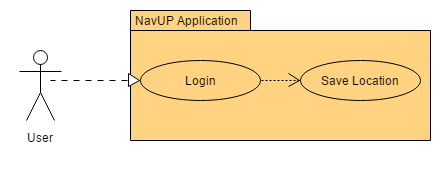
\includegraphics[width = 400px]{SaveLocation.png}
				\end{figure}
			\end{enumerate}

		\begin{table}[htb]
			\centering
			\caption{UC11 - The user logs into the application}
			\label{my-label}
			\begin{tabular}{|l|l|}
				\hline
				\textbf{Actor: User} &
				\textbf{System: NavUP}
				 \\ \hline  & 0. The NavUP system displays the user's page.
				\\ \hline
				\begin{tabular}[c]{@{}l@{}}1. The user clicks the Save Location\\ button\end{tabular}       &
				\begin{tabular}[c]{@{}l@{}}2. The system prompts the user to \\enter a description for the saved location\end{tabular}
				\\ \hline
				\begin{tabular}[c]{@{}l@{}}3. The user enters a description for the\\ saved location and confirms the action\end{tabular}       &
				\begin{tabular}[c]{@{}l@{}}4. The system saves the location and \\displays an icon over the location\end{tabular}
				\\ \hline
			\end{tabular}
		\end{table}
	
		
		%%%%%%%%%%%%%%%%%%%%%%======================   UC12    ================%%%%%%%%%%%%%%%%
		\newpage
		\subsubsection{Use Case for REQ7: Add or remove a venue}
			\begin{enumerate}
			\renewcommand{\labelenumi}{{\textbf{\arabic{enumi}.}}}
			\item Use Case ID: UC12
			\item Precondition: The administrator is logged in and wishes to add or remove a venue.
			\item Postcondition: The system is updated with the added venue.
			\item Actor-System interaction model:
				\graphicspath{ {./Images/Administrator/} }
				\begin{figure}[h]
				\caption{Use Case Diagram - UC12 Add Venue)}
				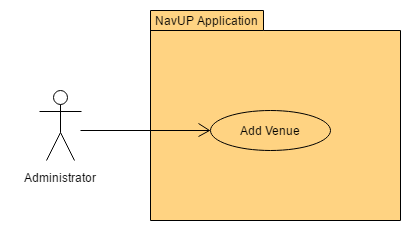
\includegraphics[width = 300px]{AddVenue.png}
				\end{figure}
		
				\graphicspath{ {./Images/Administrator/} }
				\begin{figure}[h]
				\caption{Use Case Diagram - UC12 Remove Venue)}
				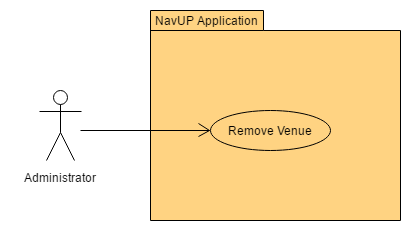
\includegraphics[width = 300px]{RemoveVenue.png}
				\end{figure}
			\end{enumerate}

		\begin{table}[htb]
			\centering
			\caption{UC12 - Add or remove venue}
			\label{my-label}
			\begin{tabular}{|l|l|}
				\hline
				\textbf{Actor: User} &
				\textbf{System: NavUP}
				 \\ \hline  & 0. The NavUP system displays the administrator's page.
				\\ \hline
				\begin{tabular}[c]{@{}l@{}}1. The adminstrator clicks on the \\add/remove venue button\end{tabular}       &
				\begin{tabular}[c]{@{}l@{}}2. The system prompts the for the location\\ and name of the new venue.\end{tabular}
				\\ \hline
				\begin{tabular}[c]{@{}l@{}}3. The administrator enters the required\\ information and confirms the action\end{tabular}       &
				\begin{tabular}[c]{@{}l@{}}4. The system saves and adds the given\\ venue\end{tabular}
				\\ \hline
			\end{tabular}
		\end{table}
		
	 
		


		%%%%%%%%%%%%%%%%%%%%%%======================   UC13    ================%%%%%%%%%%%%%%%%
		\newpage
		\subsubsection{Use Case for REQ7: Add or remove event}
			\begin{enumerate}
			\renewcommand{\labelenumi}{{\textbf{\arabic{enumi}.}}}
			\item Use Case ID: UC13
			\item Precondition: The administrator is logged in and wishes to add or remove an event.
			\item Postcondition: The system is updated with the added event.
			\item Actor-System interaction model:
				\graphicspath{ {./Images/Administrator/} }
				\begin{figure}[h]
				\caption{Use Case Diagram - UC13 Add Event)}
				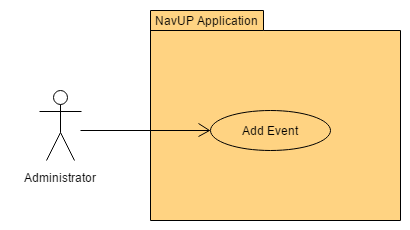
\includegraphics[width = 300px]{AddEvent.png}
				\end{figure}
		
				\graphicspath{ {./Images/Administrator/} }
				\begin{figure}[h]
				\caption{Use Case Diagram - UC13 Remove Event)}
				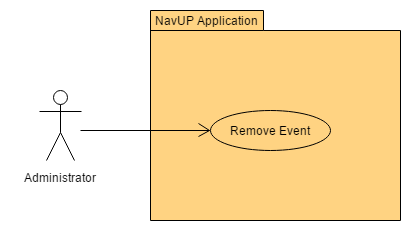
\includegraphics[width = 300px]{RemoveEvent.png}
				\end{figure}
			\end{enumerate}

		\begin{table}[htb]
			\centering
			\caption{UC13 - Add or remove event}
			\label{my-label}
			\begin{tabular}{|l|l|}
				\hline
				\textbf{Actor: User} &
				\textbf{System: NavUP}
				 \\ \hline  & 0. The NavUP system displays the administrator's page.
				\\ \hline
				\begin{tabular}[c]{@{}l@{}}1. The adminstrator clicks on the \\add/remove event button\end{tabular}       &
				\begin{tabular}[c]{@{}l@{}}2. The system prompts the for the\\ location and name of the new event.\end{tabular}
				\\ \hline
				\begin{tabular}[c]{@{}l@{}}3. The administrator enters the required \\ information and confirms the action\end{tabular}       &
				\begin{tabular}[c]{@{}l@{}}4. The system saves and adds the given\\ event\end{tabular}
				\\ \hline
			\end{tabular}
		\end{table}
		
		%%%%%%%%%%%%%%%%%%%%%%======================   UC14    ================%%%%%%%%%%%%%%%%
		\newpage
		\subsubsection{Use Case for REQ7: Update Information}
			\begin{enumerate}
			\renewcommand{\labelenumi}{{\textbf{\arabic{enumi}.}}}
			\item Use Case ID: UC14
			\item Precondition: The administrator is logged in and wishes to update the information of a venue or landmark.
			\item Postcondition: The system is updated with the added new information regarding the venue or landmark.
			\item Actor-Sytem interaction model:
				\graphicspath{ {./Images/Administrator/} }
				\begin{figure}[h]
				\caption{Use Case Diagram - UC14  Update Information)}
				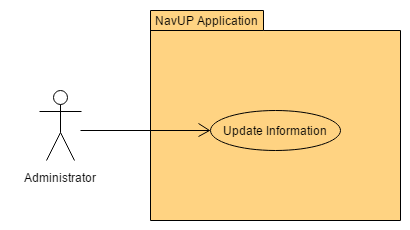
\includegraphics[width = 300px]{UpdateInfo.png}
				\end{figure}
			\end{enumerate}

		\begin{table}[htb]
			\centering
			\caption{UC14 - Update Information}
			\label{my-label}
			\begin{tabular}{|l|l|}
				\hline
				\textbf{Actor: User} &
				\textbf{System: NavUP}
				 \\ \hline  & 0. The NavUP system displays the administrator's page.
				\\ \hline
				\begin{tabular}[c]{@{}l@{}}1. The adminstrator clicks on the update \\information button\end{tabular}       &
				\begin{tabular}[c]{@{}l@{}}2.The system prompts the administrator\\ for the name or the venue or landmark for which the\\ administrator wants to update the information.\end{tabular}
				\\ \hline
				\begin{tabular}[c]{@{}l@{}}3. The administrator enters the required\\ information and confirms the action\end{tabular}       &
				\begin{tabular}[c]{@{}l@{}}4.The system prompts the administrator\\ for the new updated information for the venue.\end{tabular}
				\\ \hline
				\begin{tabular}[c]{@{}l@{}}5. The administrator enters the required\\ information and confirms the action\end{tabular}       &
				\begin{tabular}[c]{@{}l@{}}7.The system updates the application with\\ the new information\end{tabular}
				\\ \hline
			\end{tabular}
		\end{table}
		
		
		%%%%%%%%%%%%%%%%%%%%%%======================   UC15    ================%%%%%%%%%%%%%%%%
		\newpage
		\subsubsection{Use Case for REQ7: Add or remove goals}
			\begin{enumerate}
			\renewcommand{\labelenumi}{{\textbf{\arabic{enumi}.}}}
			\item Use Case ID: UC15
			\item Precondition: The administrator is logged in and wishes to add or remove a goal.
			\item Postcondition: The system is updated with the new goals information.
			\item Actor-System interaction model:
				\graphicspath{ {./Images/Administrator/} }
				\begin{figure}[h]
				\caption{Use Case Diagram - UC15 Add Goals)}
				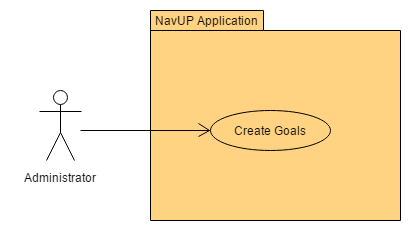
\includegraphics[width = 300px]{AddGoals.png}
				\end{figure}
		
				\graphicspath{ {./Images/Administrator/} }
				\begin{figure}[h]
				\caption{Use Case Diagram - UC15  Remove Goals)}
				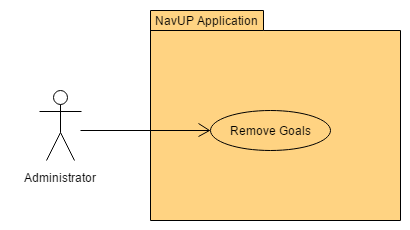
\includegraphics[width = 300px]{RemoveGoals.png}
				\end{figure}
			\end{enumerate}

		\begin{table}[htb]
			\centering
			\caption{UC15 - Add or remove goals}
			\label{my-label}
			\begin{tabular}{|l|l|}
				\hline
				\textbf{Actor: User} &
				\textbf{System: NavUP}
				 \\ \hline  & 0. The NavUP system displays the administrator's page.
				\\ \hline
				\begin{tabular}[c]{@{}l@{}}1. The adminstrator clicks on the\\ add/remove goals button\end{tabular}       &
				\begin{tabular}[c]{@{}l@{}}2. The system prompts the for the\\ requirements and name of the new goals etc.\end{tabular}
				\\ \hline
				\begin{tabular}[c]{@{}l@{}}3. The administrator enters the required\\ information and confirms the action\end{tabular}       &
				\begin{tabular}[c]{@{}l@{}}4. The system updates the application with\\ the new ionformation\end{tabular}
				\\ \hline
			\end{tabular}
		\end{table}
		
		\graphicspath{ {./Images/AdjacencyMatrix/} }
		\begin{figure}
		
\includegraphics[width=16cm, height=4cm]{Adjaceny-Matrix-1.png}
		\caption{Traceability Matrix 1}
		\end{figure}

		\begin{figure}
		
\includegraphics[width=16cm, height=4cm]{Adjacency-Matrix-2.png}
		\caption{Traceability Matrix 2}
		\end{figure}
	
	\newpage
	\subsection{Quality Requirements}
				A system of the complexity and scale of NavUP must meet specific quality requirements such as:
				
				\begin{enumerate}
				\renewcommand{\labelenumi}{{\textbf{\arabic{enumi}.}}}
				\item Performance - the system must handle a possibility of over 50000 users simultaneously and still perform the core functionality without failure.
				\item Reliability - the sytem should perform its functionality reliably,  most importantly the navigational requirements.
				\item Usability - the system should be easy to use while sporting an aesthetic and ergonomic interface.
				\item Integrability - the system should allow for additional features and modules to be added easily.
				\end{enumerate}
				

			\subsection{Access Channel Requirements}
				From the typical user's perspective,  approximately 60000 students and staff,  the NavUP system will largely be focused on mobile devices such as Android or iOS smartphones.
				These devices,  will make use of location services and internet capabilities to send and recieve data to and from access channels and servers using mobile data, 
				Wi-Fi signals,  crowdsourcing and geolocation systems such as GPS and GIS. The campus Wi-Fi network will be the main form of system access as the signal
				strength covers most of the large area the University spans,  and will help location accuracy indoors where the mobile devices may struggle to find decent mobile
				and location based signals.

			
			\subsection{Integration Requirements}
				The NavUP system will be implemented simultaneously by all the students enrolled in COS 301,  it is therefore imperative that the system complies to a low coupling and high cohesion standard.
			\subsection{Architecture Constraints}
				The clients have specified the use of technologies such as GIS,  UI/UX,  Mobile Development (Android/iOS),   Real-time Data Analysis,  Data Streaming and
				Persistence,  and a large focus on the use of Wi-Fi Networking to boost the system's accuracy. A module that supplies targeted delivery of information was also requested hence an intelligent program is also required.
				
			\subsection{User Interface}
				The user interface is likely to be used by students and staff alike,  and many visitors to the campus,  the interface therefore should be friendly and easy to use for all ages. The interface should include functionality for users to login and create 						personal profiles
				so that they can use the rewards system and access other functionality. There should also be different interface for administrative users who must be able to create point of interest and update activities and update and capture location data.



\end{document}